\documentclass[a4paper, dvipsnames]{article}

\usepackage[T1]{fontenc}
\usepackage{geometry}
\geometry{
  left=2cm,
  right=2cm,
  top=4cm,
  bottom=4cm,
  bindingoffset=5mm
}

\usepackage{amssymb} 
\usepackage{amsmath}
\usepackage{amsthm}
\usepackage[utf8]{inputenc}
\usepackage[T1]{fontenc}
\usepackage{lmodern}
\usepackage{ngerman}
\usepackage{scrlayer-scrpage}
\usepackage{ulem}
\usepackage{xcolor}
\usepackage{graphicx}
\usepackage{listings}

\lstset{
language=Java,
aboveskip=3mm,
belowskip=3mm,
showstringspaces=false,
keywordstyle=\color{OliveGreen},
commentstyle=\color{gray},
breaklines=true,
breakatwhitespace=true,
tabsize=4
}

\pagestyle{scrheadings}

\ihead{Gruppe 10}
\chead{Logische Programmierung}
\ohead{\pagemark}

\setlength{\parindent}{0pt}


\begin{document}

{ \hspace{7,7cm}{\bfseries{Serie 1}}  {\hspace{6,0cm}{Gruppe 10}}\\

Adnan Alyousfi, 218205332, Informatik\\
Dirk Peglow, Informatik\\
Nils Henrik Seitz, 218205308, Informatik\\
Lorka Trad, Informatik\\
Nico Trebbin, 218204402, Informatik\\

\uline{\bfseries{Aufgabe 1}}\\

{\bfseries 1.A}\\

unify({\color{red}f}(g(2, 3), Y ), {\color{red}f}(X, f(2)))\quad$\theta = \{\}$\\
unify(f({\color{red}g(2, 3)}, Y ), f({\color{red}X}, f(2)))\quad$\theta = \{X = g(2,3)\}$\\
unify(f(g(2, 3), {\color{red}Y} ), f(g(2, 3), {\color{red}f(2)}))\quad$\theta = \{X = g(2,3), Y = f(2)\}$\\
unify(f(g(2, 3), f(2) ), f(g(2, 3), f(2)))\quad$\theta = \{X = g(2,3), Y = f(2)\}$\\
$\theta = \{X = g(2,3), Y = f(2)\}$ (Allgemeinster Unifikator)\\

{\bfseries 1.B}\\

unify\{{\color{red}g}(X), {\color{red}f}(X)\}\quad$\theta = \{\}$ - Nicht unifizierbar, da die Funktoren unterschiedlich sind.\\

{\bfseries 1.C}\\

unify({\color{red}f}(X, g(Y, Y )), {\color{red}f}(g(Y, Y ),X))\quad$\theta = \{\}$\\
unify(f({\color{red}X}, g(Y, Y )), f({\color{red}g(Y, Y )},X))\quad$\theta = \{X = g(Y,Y)\}$\\
unify(f(g(Y,Y), \color{red}g(Y, Y )}), f(g(Y, Y ),{\color{red}g(Y,Y)})\quad$\theta = \{X = g(Y,Y)\}$\\
unify(f(g(Y,Y), g(Y, Y )), f(g(Y, Y ),g(Y,Y))\quad$\theta = \{X = g(Y,Y)\}$\\
$\theta = \{X = g(Y,Y)\}$ (Allgemeinster Unifikator)\\

{\bfseries 1.D}\\

unify({\color{red}f}(X, g(Y, Y )), {\color{red}f}(g(Y, Y ), Y ))\quad$\theta = \{\}$\\
unify(f({\color{red}X}, g(Y, Y )), f({\color{red}g(Y, Y )}, Y ))\quad$\theta = \{X = g(Y, Y)\}$\\
unify(f(g(Y, Y), g(Y, Y )), f(g(Y, Y ), Y ))\quad$\theta = \{X = g(Y, Y)\}$\\ - Nicht unifizierbar, da Y im Term g(Y, Y) auftaucht. Beim unifizieren würde dies zu einer Endlosschleife führen.\\

\newpage

\uline{\bfseries{Aufgabe 2}}\\
{\bfseries 2.B}\\
\begin{center}
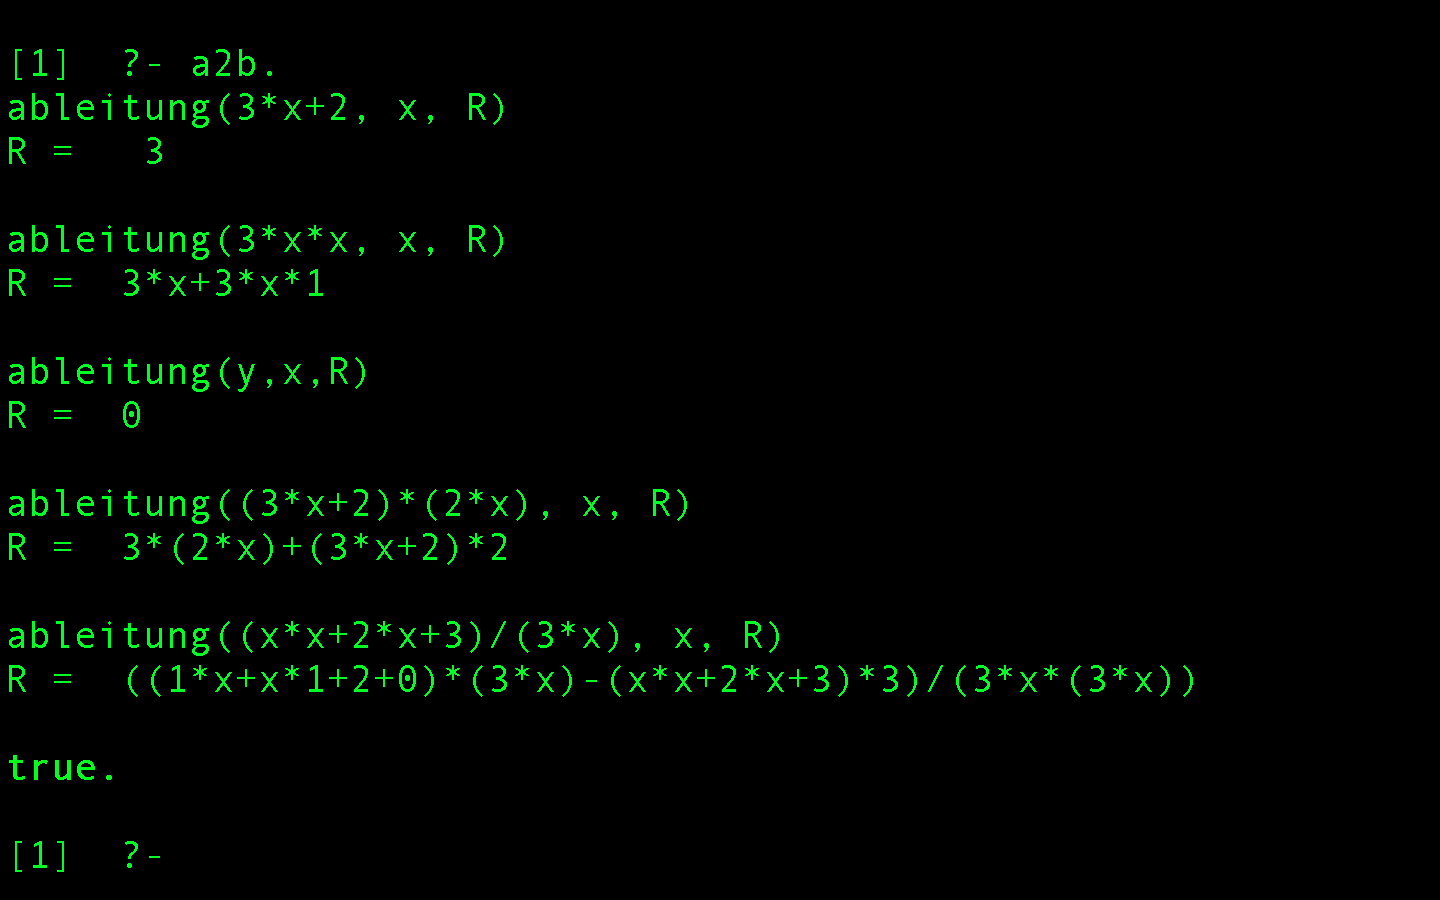
\includegraphics[width=0.6\textwidth]{Data/A2/1.png}
\end{center}

\uline{\bfseries{Aufgabe 3}}\\
R - running, D - damaged, I - ignition , F - fuel, B - battery, P - plug\\
\\
{\bfseries 3.A}\\
\texttt{D;R :- I,F } $\equiv$ \texttt{ R :- I,F,not(D)}\\
 $I \wedge F \rightarrow D \vee R \equiv I \wedge F \wedge \neg D \rightarrow R$\\
$\neg (I \wedge F) \vee D \vee R \equiv \neg (I \wedge F \wedge \neg D) \vee R$\\
$\neg I \vee \neg F \vee D \vee R \equiv \neg I \vee  \neg F \vee  D \vee R$\\

{\bfseries 3.B}\\
$HB = \lbrace$\texttt{running,  damaged,  ignition ,  fuel,  battery,  plug}$ \rbrace$\\

{\bfseries 3.C}\\
$I = \lbrace \emptyset, R, D, I, B, F, P, $\\
$RD, RI, RB, RF, RP, DI, DB, DF, DP, IB, IF, IP, BF, BP, FP$\\
$RDI, RDB, RDF, RDP, RIB, RIF, RIP, RBF,RBP,RFP,$\\
$DIB, DIF, DIP, DBF, DBP, DFP, IBF, IBP, IFP, BFP, $\\
$RDIB, RDIF, RDIP, RDBF, RDBP, RDFP,$\\
$ RIBF, RIBP, RIFP, RBFP, DIBF, DIBP, DIFP, DBFP, IBFP$\\
$RDIBF, RDIBP, RDIFP, RDBFP, RIBFP, DIBFP, RDIBFP\rbrace$\\

\texttt{fuel.}: Alle Modelle müssen $F$ enthalten.:\\
$I = \lbrace F, RF, DF, IF, BF, FP$\\
$RDF, RIF, RBF,RFP, DIF, DBF, DFP, IBF, IFP, BFP, $\\
$RDIF,  RDBF,RDFP,RIBF,  RIFP, RBFP, DIBF, DIFP, DBFP, IBFP$\\
$RDIBF, RDIFP, RDBFP, RIBFP, DIBFP, RDIBFP\rbrace$\\

\texttt{battery.}: Alle Modelle müssen $B$ enthalten.:\\
$I = \lbrace  BF,  RBF,DBF,  IBF, BFP, $\\
$  RDBF,RIBF,  RBFP, DIBF,  DBFP, IBFP$\\
$RDIBF,  RDBFP, RIBFP, DIBFP, RDIBFP\rbrace$\\
\newpage
\texttt{:- plug.}: Kein Modell darf $P$ enthalten.:\\
$I = \lbrace  BF,  RBF,DBF,  IBF, RDBF,RIBF, DIBF , RDIBF \rbrace$\\

\texttt{ignition :- plug, battery.}: Wenn $P \wedge B$, dann $I$ (aber $P$ wurde eben überall entfernt).:\\
$I = \lbrace  BF,  RBF,DBF,  IBF, RDBF,RIBF, DIBF , RDIBF \rbrace$\\

\texttt{running :- ignition, fuel,not(damaged).}: Wenn $I \wedge F \wedge \neg D$, dann $R $ (intendiertes Modell).:\\
$I = \lbrace  BF,  RBF,DBF,  RDBF,RIBF,DIBF , RDIBF  \rbrace =$ minimales Modell\\


{\bfseries 3.D}\\
\texttt{F.\\
B.\\
:- P.\\
I :- B, P.\\
R:- I,F,not(D). ($\equiv$ D;R :- I,F , siehe 3.A )}\\

\textbf{Direkter Beweis: }\\
zu zeigen: \texttt{ D;R :- P.} \\
$$\frac{\texttt{D;R :- I,F. \; \; F. }}{\texttt{D;R :- I.}}$$
$$\frac{\texttt{D;R :- I. \; \; I :- B,P. }}{\texttt{D;R :- B,P.}}$$
$$\frac{\texttt{D;R :- B,P. \; \; B. }}{\texttt{D;R :- P.}}$$

\textbf{Refutationsbeweis:}\\
Negation der Zielklausel: $\neg$(\texttt{ D;R :- P.} )\\
$\equiv \neg ( D \vee R \vee  \neg P )$\\
$\equiv \neg  D \wedge \neg  R \wedge  P $\\
$\equiv$ \texttt{:- R.} und \texttt{:- D.} und \texttt{P.} \\

1. \texttt{:- R.  $\;\;\;$        R :- I,F,not(D).}\\
2. \texttt{:- I,F,not(D).  $\;\;\;$        :- D.}\\
3. \texttt{:- I,F.  $\;\;\;$       I :- B,P.}\\
4. \texttt{:- B,P,F. $\;\;\;$       B.}\\
5. \texttt{:- P,F. $\;\;\;$       F.}\\
6. \texttt{:- P.  $\;\;\;$       P.}\\
7. \texttt{       [] }\\





\end{document}